%! Author = fabian
%! Date = 21.11.21

% Preamble
\documentclass[a4paper]{article} % Uses article class in A4 format

%----------------------------------------------------------------------------------------
%	FORMATTING
%----------------------------------------------------------------------------------------

\addtolength{\hoffset}{-2.25cm}
\addtolength{\textwidth}{4.5cm}
\addtolength{\voffset}{-3.25cm}
\addtolength{\textheight}{5cm}
\setlength{\parskip}{0pt}
\setlength{\parindent}{0in}


%----------------------------------------------------------------------------------------
%	PACKAGES AND OTHER DOCUMENT CONFIGURATIONS
%----------------------------------------------------------------------------------------

\usepackage[utf8]{inputenc} % Use UTF-8 encoding
%\usepackage{microtype} % Slightly tweak font spacing for aesthetics

\usepackage[english]{babel} % Language hyphenation and typographical rules

\usepackage{amsthm, amsmath, amssymb, bm} % Mathematical typesetting
\usepackage{float} % Improved interface for floating objects
%\usepackage[final, colorlinks = true,
%linkcolor = black,
%citecolor = black]{hyperref} % For hyperlinks in the PDF
\usepackage{graphicx, multicol} % Enhanced support for graphics
\usepackage{subcaption}
\usepackage{xcolor} % Driver-independent color extensions
%\usepackage{marvosym, wasysym} % More symbols
%\usepackage{rotating} % Rotation tools
%\usepackage{censor} % Facilities for controlling restricted text!
%\usepackage{booktabs} % Enhances quality of tables
%\usepackage{censor} % Facilities for controlling restricted text!
%\usepackage{booktabs} % Enhances quality of tables
\usepackage{listings}
\usepackage{caption}

%\usepackage{csquotes} % Context sensitive quotation facilities
%\usepackage[yyyymmdd]{datetime} % Uses YEAR-MONTH-DAY format for dates
%\renewcommand{\dateseparator}{-} % Sets dateseparator to '-'

\usepackage{fancyhdr}
\usepackage{amsmath} % Headers and footers
\pagestyle{fancy} % All pages have headers and footers
\fancyhead{}\renewcommand{\headrulewidth}{0pt} % Blank out the default header
\fancyfoot[L]{} % Custom footer text
\fancyfoot[C]{} % Custom footer text
\fancyfoot[R]{\thepage} % Custom footer text

%\newcommand{\note}[1]{\marginpar{\scriptsize \textcolor{red}{#1}}} % Enables comments in red on margin
\DeclareMathOperator*{\argmax}{argmax}
\DeclareMathOperator*{\argmin}{argmin}
%----------------------------------------------------------------------------------------

% Document
\begin{document}
%----------------------------------------------------------------------------------------

%	TITLE SECTION
    \title{Title} % Article title
    \fancyhead[C]{}
    \hrule \medskip % Upper rule
    \begin{minipage}{0.295\textwidth} % Left side of title section
        \raggedright
        TTK4255\\ % Your lecture or course
        \footnotesize % Authors text size
        \hfill\\
        Fabian Höldin \\
         Sindre {\O}versveen% Your name, your matriculation number
    \end{minipage}
    \begin{minipage}{0.4\textwidth} % Center of title section
        \centering
        \large % Title text size
        Robotic Vision \\ % Assignment title and number
        \normalsize % Subtitle text size
        Final project: Visual localization\\ % Assignment subtitle
    \end{minipage}
    \begin{minipage}{0.295\textwidth} % Right side of title section
        \raggedleft
        \today\\ % Date
        \footnotesize % Email text size
        \hfill\\
        % Your email
    \end{minipage}
    \medskip\hrule % Lower rule
%----------------------------------------------------------------------------------------
%	ARTICLE CONTENTS
%----------------------------------------------------------------------------------------
    
\section{Camera calibration}

    \subsection*{Task 1.1}

    \begin{figure}[h]
        \center
        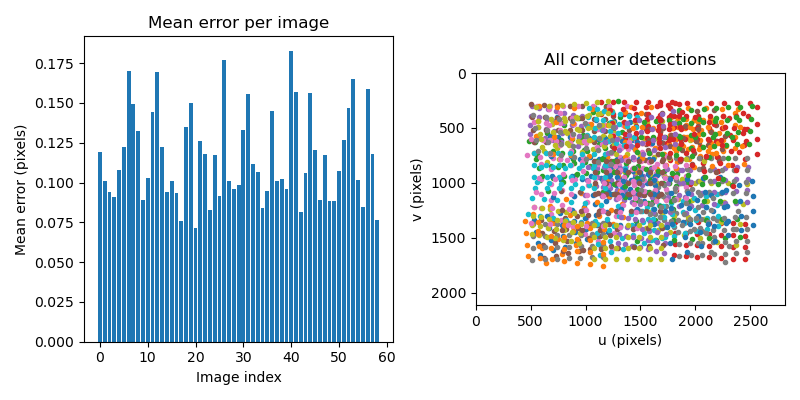
\includegraphics[width= \linewidth]{calibrationResult}
        \caption{Results of the camera calibration}
    \end{figure}

    \begin{description}
        \item [a)] There are several potential reasons that would result in significantly higher errors.
                This could be due to a strong tilt that often times also comes with changes of illumination.
                The visual tilting effect can also occur if the checkerboard is at the edge of the camera frame even though it is parallel to the image plane.
                To test this one could take a subset of pictures with a high visual tilting and calculate the error.
                If it applies there should be a significant difference to the error of the whole set.
        \item [b)] In general the accuracy looks quite alright.
                Whereas you can notice that it gets worse the closer you get to a corner.
                There you can still observe some distortion. 
                So if you were to extend the calibration picture database, it should be with pictures close to the image frame and especially the corners.
    \end{description}

    \subsection*{Task 1.2}

    \begin{figure}[H]
        \centering
        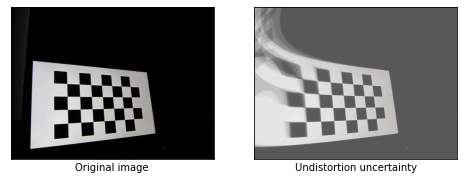
\includegraphics[width= 0.7 \linewidth]{deviation}
    \end{figure}
    For the code see 'task\_handinds.ipynb'.
    \begin{description}
        \item [a)] When the purpose is to build intuition for the uncertainty in distortion parameters, using the calibration images is not necessary.
                After all, performing undistort() with 'incorrect' coefficients is equivical to performing distortion - the variant strength of which represents the uncertainty.

        \item [b)] It as our opinion that the settings that keeps cropping and scaling to a minimum, and keeps invalid pixels, are preferable.
                This is because the variations in black borders makes changes in the image easier to identify

        \item [c)] The effects of undistortion is hardly noticeable.
                Amplifying the standard deviation by a factor of 100 confirms that there is indeed some effects, and that the majority of this is near the corners of the image.
                This is intuitive, as its further from the 'center' of radial distortion, and the conclusion from 1.1b.
    \end{description}


\section{Model creation}

    \subsection*{Task 2.1}
    Implemented in 'example\_match\_features.py'.
    \begin{description}
        \item [a)]  \hfill \\
            \begin{figure}[H]
                \center
                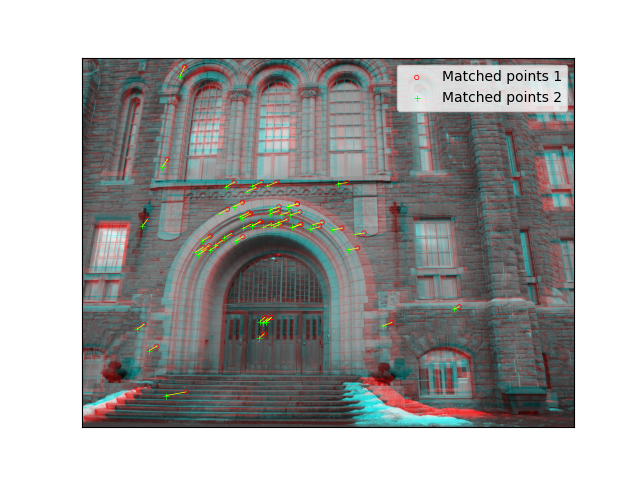
\includegraphics[width= 0.7\linewidth]{Correspondence}
                \caption{Best 50 correspondences by descriptor distance.}
            \end{figure}
            \begin{figure}[H]
                \center
                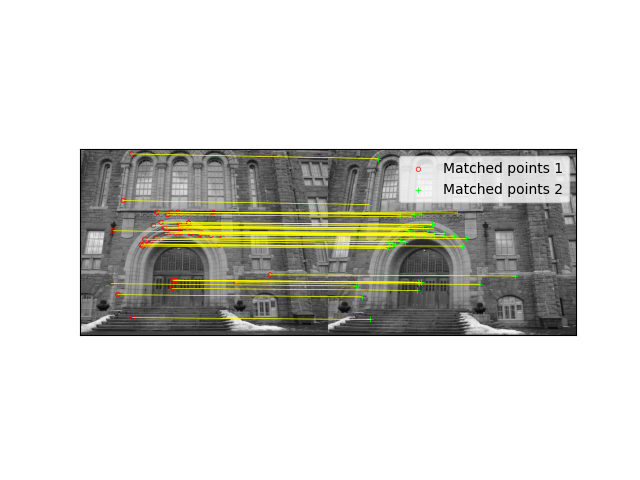
\includegraphics[width= \linewidth]{Matches}
                \caption{50 matches side by side.}
                \end{figure}
        \item [b)]  \hfill \\
            \begin{figure}[H]
                \center
                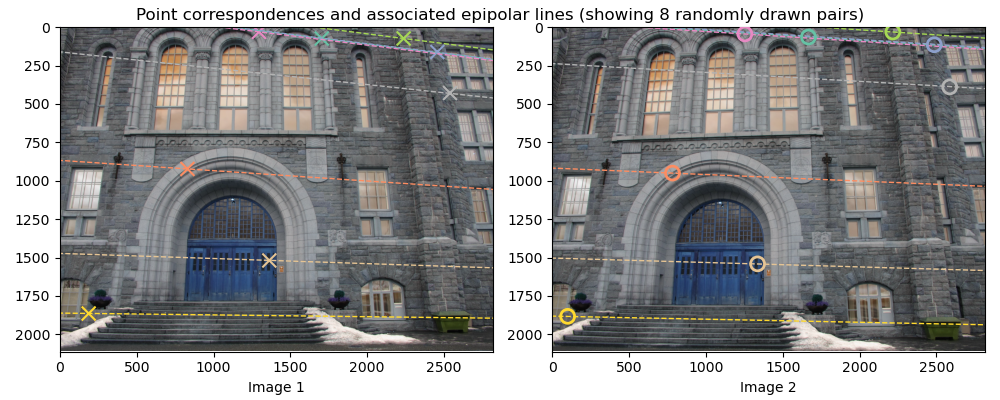
\includegraphics[width= \linewidth]{epipolarLines}
                \caption{8 inlier correspondences with their epipolar lines.}
            \end{figure}
        \item [c)]  In the included figures we used a maximum ratio og 0.9 and set the uniqueness parameter to true.
                    By playing around with these parameters we found that decreasing the max ratio results in way fewer matches, it also minimizes wrong matches.
                    Beside of the already pre-implemented knn distance metric we also tried out an ORB detector using the Hamming distance (commented out).
        \item [d)]  For estimating the relative pose and the 3D point coordinates we simply reused the RANSAC approach from HW5.
                    This gave us a total of 10966 inliers out of 12191 matches.
                    In the following figure you can see the point-cloud of the best solution.
            \begin{figure}[h]
                \center
                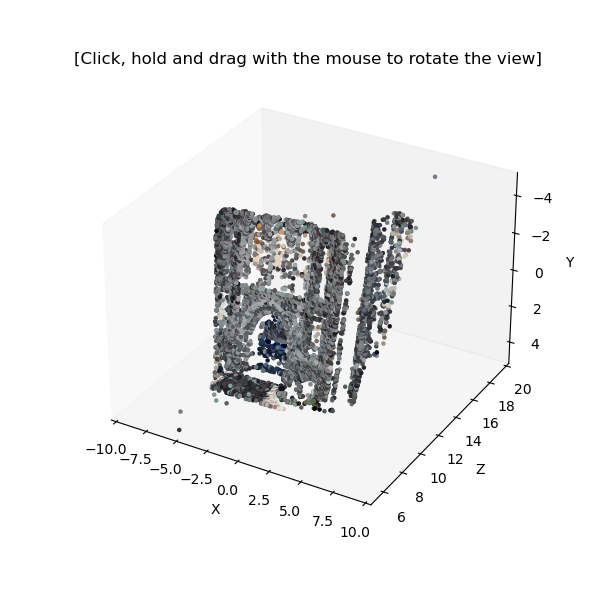
\includegraphics[width= 0.7 \linewidth ]{3D_point_cloud}
                \caption{Reconstructed 3D point cloud.}
            \end{figure}
        \item [e)]  The above point cloud consists of 10964 visible of 10966 total inlieres what is the pest found solution.
                    These reconstructions have been saved for later usage together with their correspondent feature descriptors.
    \end{description}
    
    \subsection*{Task 2.2}

    Bundle adjusment refers to a general method of reconstruction problems, and can in this context be used to refine an existing, suboptimal estimation of camera motion and 3D structure.
    It works by solving a minimization problem with the square reprojection error. The parameters are the 3D coordinates for the <...> points and the camera parameters (rotation, translation and intrinsics).
    The objective function is
    $$ E=\sum_{i=1}^m ||P_i \widetilde{\underline{\textbf{x}}} - \widetilde{\underline{\textbf{x}}}'||$$
    If using the "Sparse BA" formulation, minimizing with Levenberg-Marquardt, one can leverage the sparsity of the Jacobian to increase computational efficiency.
    The Jacobian contains an substructure relating to each camera angle (motion) and each measurement point (3D coordinate).
    If there are for instance 3 cameras and 4 points, the Jacobian's structure would be as such:
    \begin{figure}[H]
        \centering
        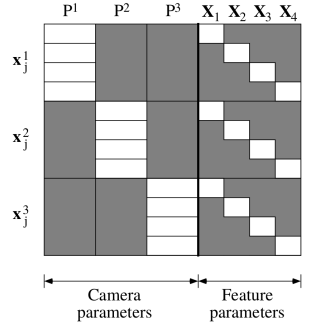
\includegraphics[width= 0.3 \linewidth]{sparse_bundle}
        \caption{Sparse bundle adjustment matrix structure.}
    \end{figure}
    
    \subsection*{Task 2.3}
    To scale the 3D coordinate system to a meters, we need to figure out the scaling factor. 
    This can be obtained by knowing the real distance between 2 points (in meters) and dividing that by the measured distance on the current 3D representation.  
    Applying this scaling factor to all the points in the system will result in the axis being in meters.

\section{Localization and uncertainty analysis}
    \subsection*{Task 3.2}
    \begin{figure}[H]
        \center
        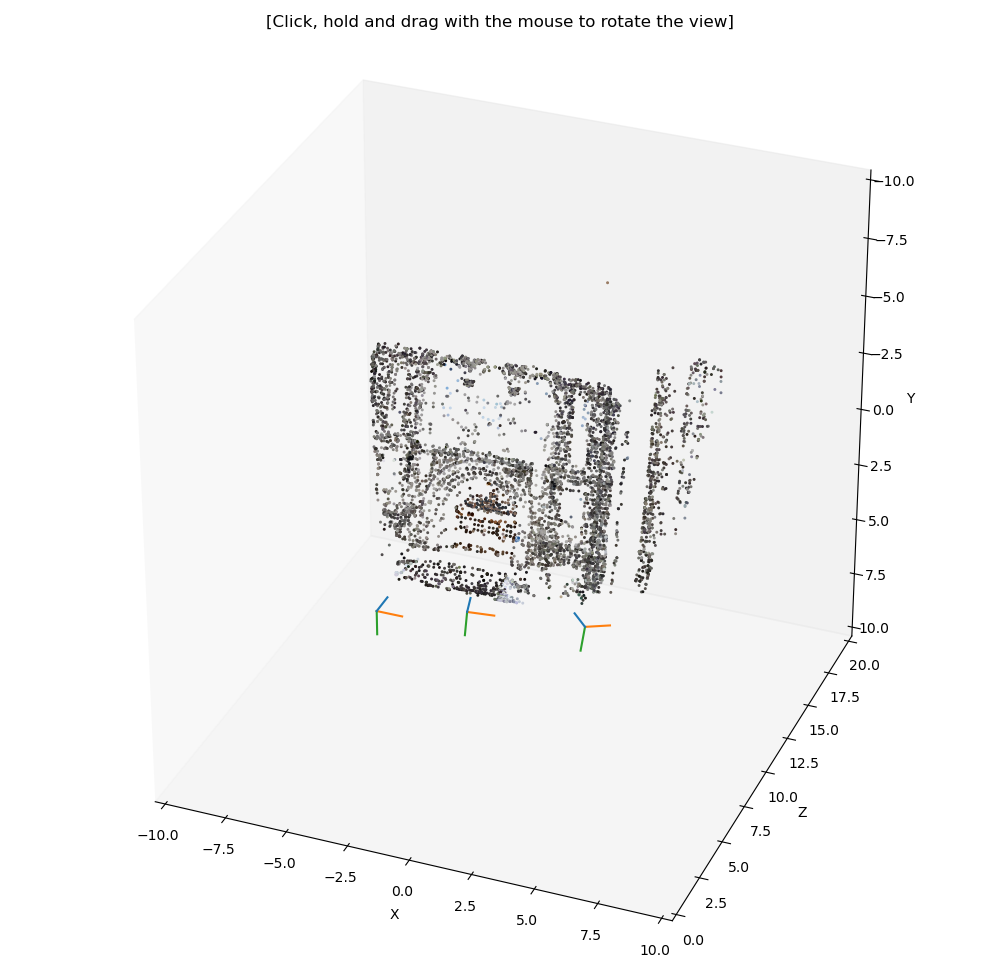
\includegraphics[width= 0.7 \linewidth]{cam_pos}
        \caption{The figure shows the generated point point cloud and three located camera poses of: IMG\_8207, IMG\_8215, IMG\_8228.}
    \end{figure}
    As can be seen in the above figure, our localization works.
    If you look at the pictures you can verify that the estimated poses and locations fit.
    In general one can say the further a picture is taken from the initial ones, the less matching points are found and the reprojection error increases.
    On the other hand this means that if you try to localize one of the initial images, you find loads of matches and the error is very low.
    The figures below you can see one inlier point cloud of an initial image and one where the camera is far away.

    \begin{figure}[H]
        \centering
        \begin{subfigure}[b]{0.45\textwidth}
         \centering
         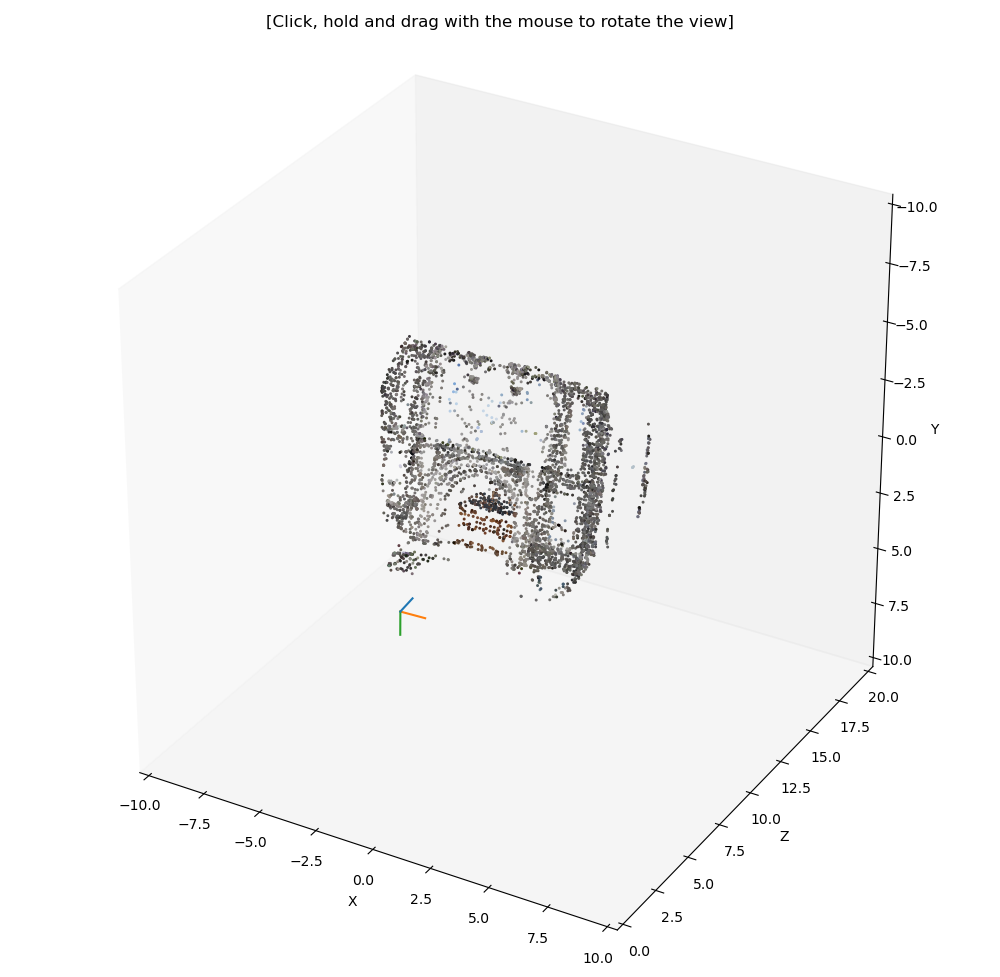
\includegraphics[width=\textwidth]{matches_many}
         \caption{IMG\_8210: One of the inital pictures. Therefor a lot of inliers are found. }
     \end{subfigure}
     \hfill
     \begin{subfigure}[b]{0.45\textwidth}
         \centering
         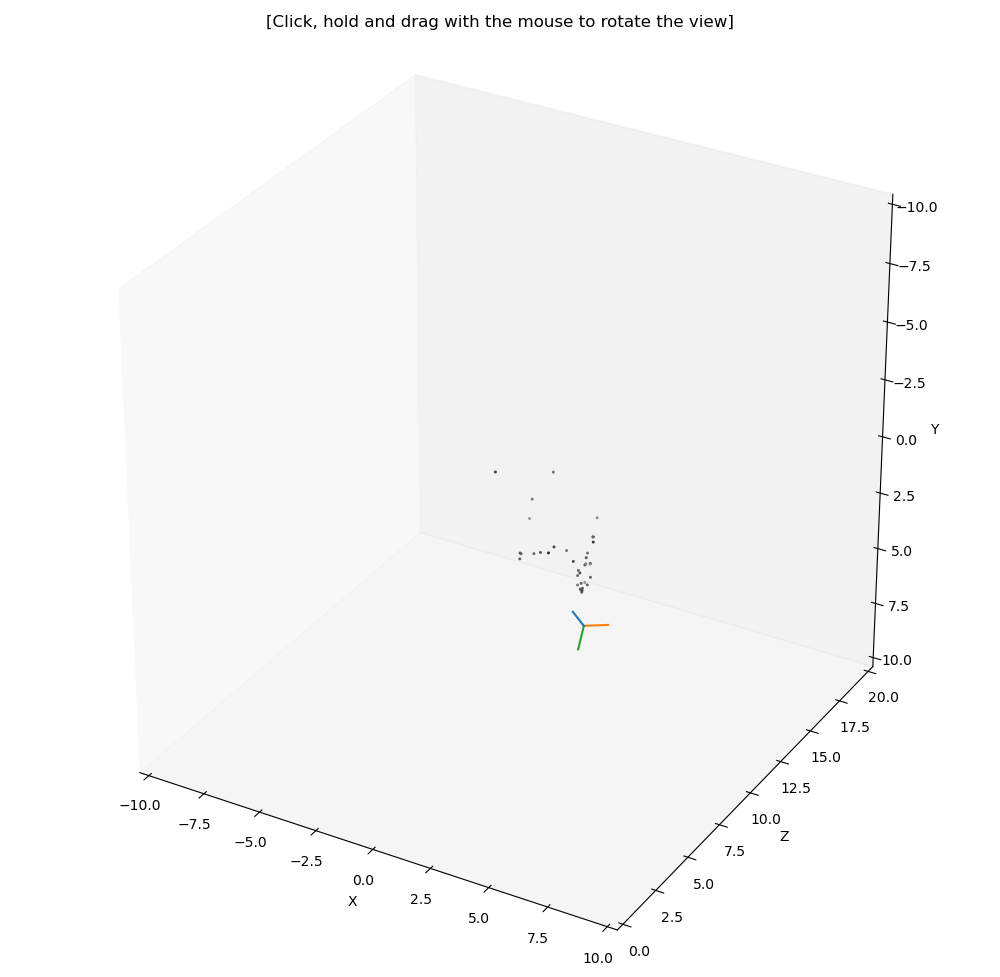
\includegraphics[width=\textwidth]{matches_few}
         \caption{IMG\_8216: Picture is made far from the side. Only 35 inliers are found. }
     \end{subfigure}
    \end{figure}

    \subsection*{Task 3.3}
    The amount of inliers matches and the reprojection error already give a first estimate how good the localization is.
    Another property that can be used for further validation are the color values.
    Whereas for this it might be necessary to perform histogram equalization before using the images.
    
    \subsection*{Task 3.4}
    Pose parameter std. deviations:\\
    \begin{tabular}{l|lll}
        image & IMG\_8207 & IMG\_8215 & IMG\_8228 \\
        \hline
        Rotations: & [9.6468e-4 6.3234e-4 3.7941e-4] & [2.2752e-3 1.4374e-3 1.0056e-3] & [5.5933e-4 4.5021e-4 3.0571e-4]\\
        Translations: & [0.1107 0.1508 0.0472] & [0.1210 0.2374 0.1809] & [0.0607 0.0677  0.0308]\\
    \end{tabular}

    \subsection*{Task 3.5}
    Pose parameter std. deviations with weighting:\\
    \begin{tabular}{l|lll}
        image & IMG\_8207 & IMG\_8215 & IMG\_8228 \\
        \hline
        Rotations: & [7.2157e-7 3.0878e-7 2.7816e-7] & [5.5433e-6 1.9041e-6 2.4646e-6]  & [6.0389e-7 2.7063e-7 2.9049e-7] \\
        Translations: & [8.2479e-4 0.2137  1.3348e-3] & [0.0118  0.1006 0.0125] & [5.4322e-3 0.0696 2.0152e-3]
    \end{tabular}

    Even though the standard deviations are improving with weighting, you can not really spot a difference in the figures.

    \begin{figure}[H]
        \centering
        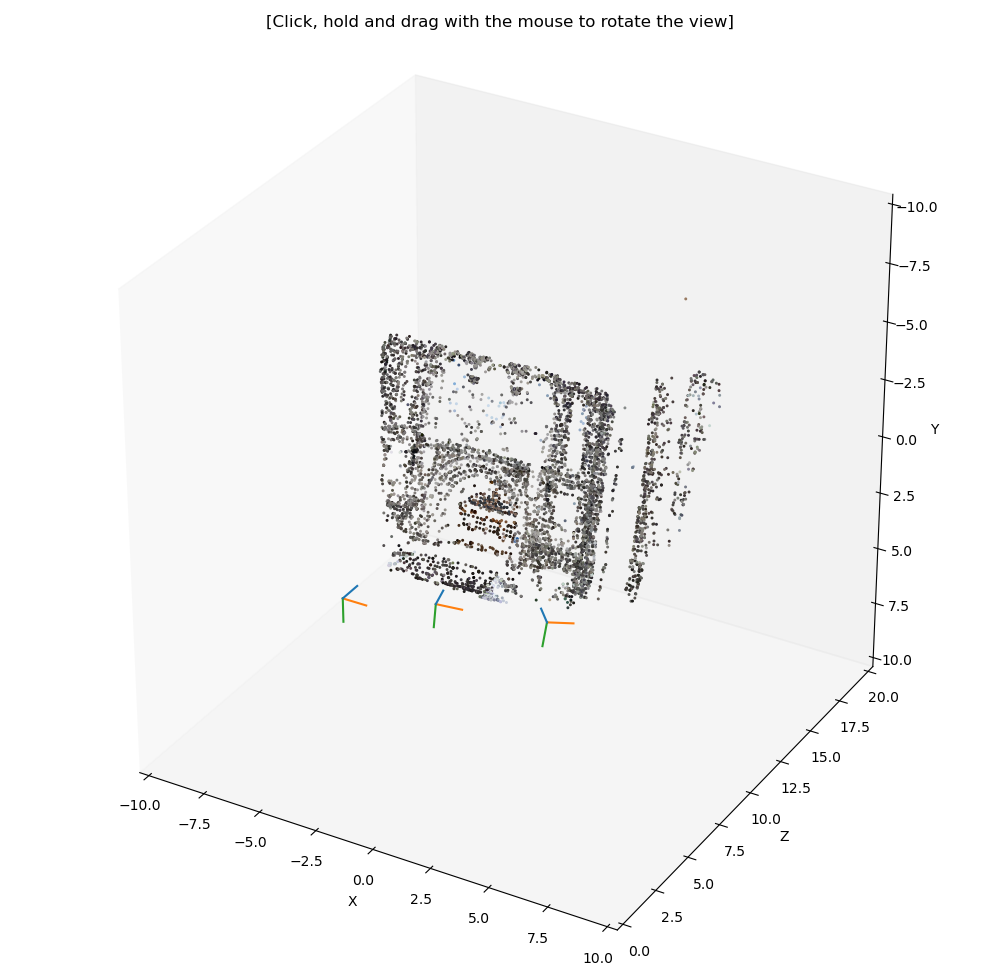
\includegraphics[width= 0.7 \linewidth]{cams_weighted}
        \caption{Localized images IMG\_8207, IMG\_8215, IMG\_8228 with weighting.}
    \end{figure}

\end{document}
